\section{Вычислительный эксперимент} \label{section:experiments}

Целью данного раздела является эмпирическая проверка эффективности предложенного алгоритма \textsc{No Full Grad SARAH} на задачах классификации изображений. Были проведены вычислительные эксперименты на следующих датасетах:
\begin{itemize}
    \item \textsc{CIFAR-10} и \textsc{CIFAR-100} с использованием архитектуры ResNet-18;
    \item \textsc{Tiny ImageNet} с использованием модели Swin Transformer.
\end{itemize}

Во всех экспериментах обучение осуществлялось  с размером батча 128. Параметр регуляризации веса был установлен как $\lambda_1 = 5 \times 10^{-4}$. Для каждой модели фиксировались метрики качества на обучающей и тестовой выборках: кросс-энтропийная функция потерь и точность. Метрики визуализировались в зависимости от числа эквивалентных вызовов полного градиента.

\subsection{Результаты на \textsc{CIFAR-10} с использованием ResNet-18}

\begin{figure}[H]
\centering
\begin{tabular}{cc}
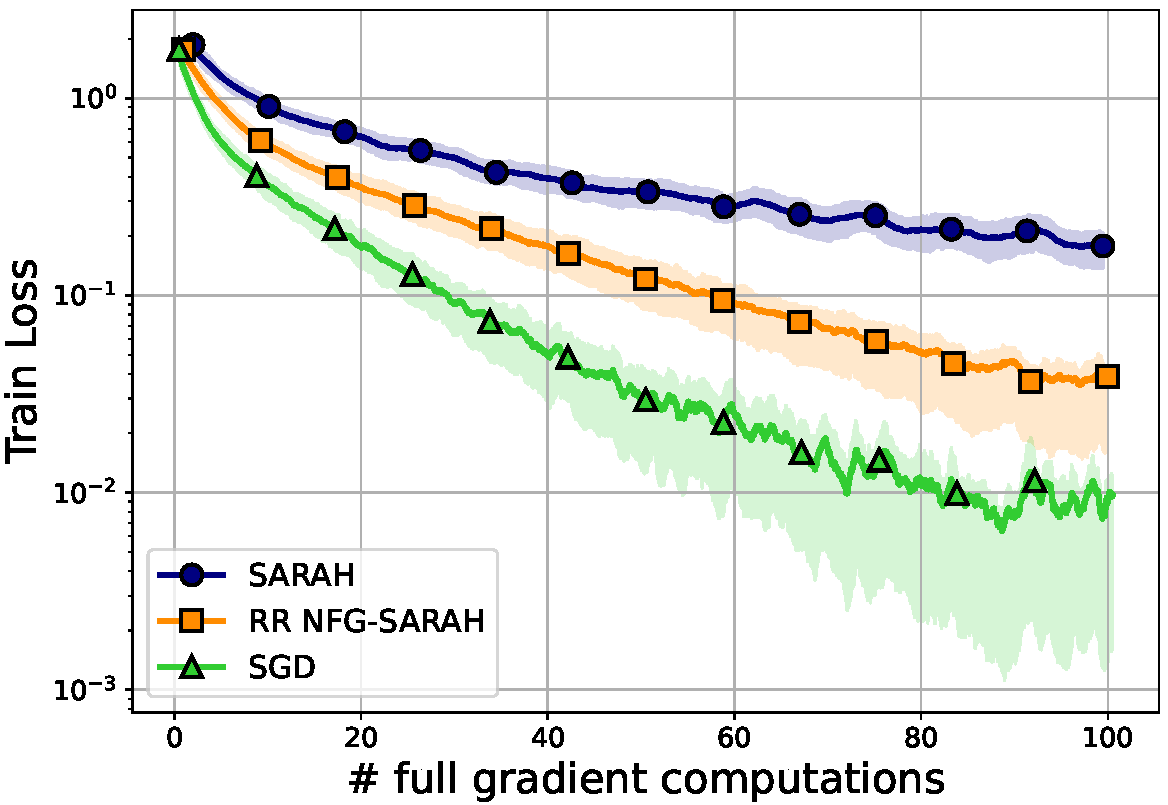
\includegraphics[width=0.45\textwidth]{plots/sarah_10-train-loss_compressed.pdf} &
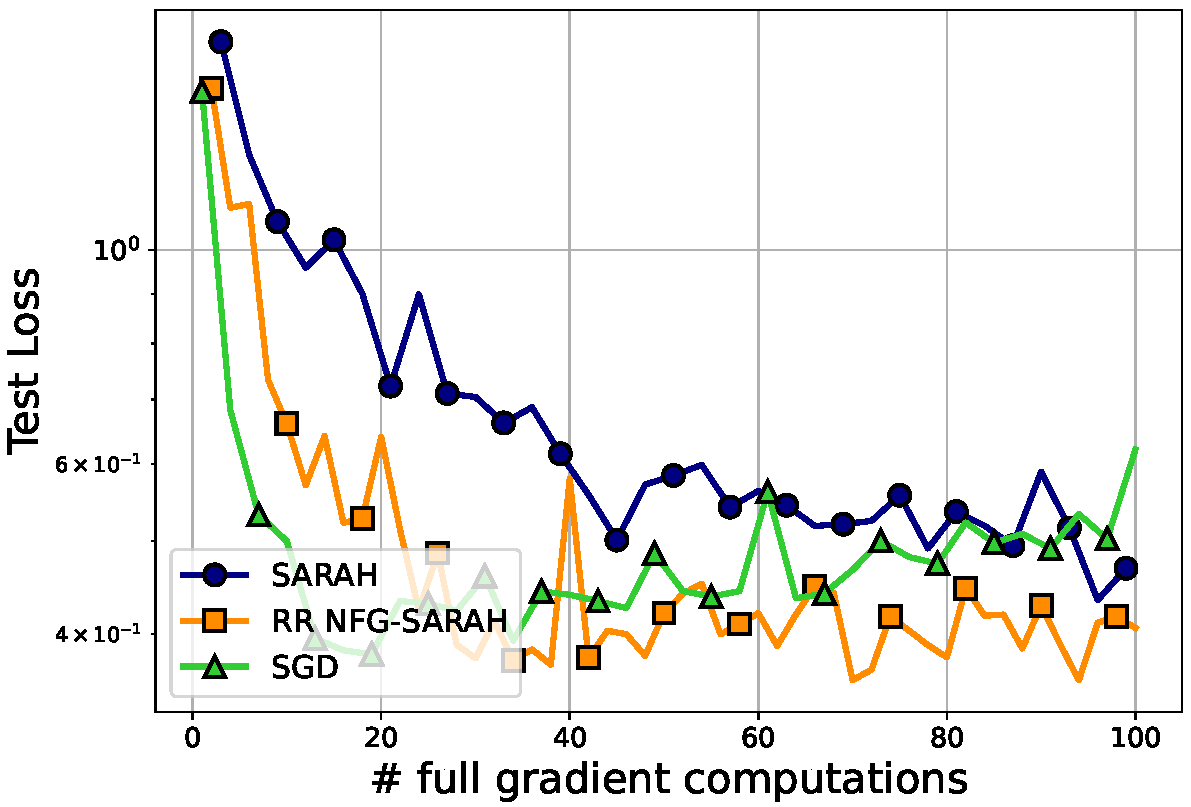
\includegraphics[width=0.45\textwidth]{plots/sarah_10-test-loss_compressed.pdf} \\
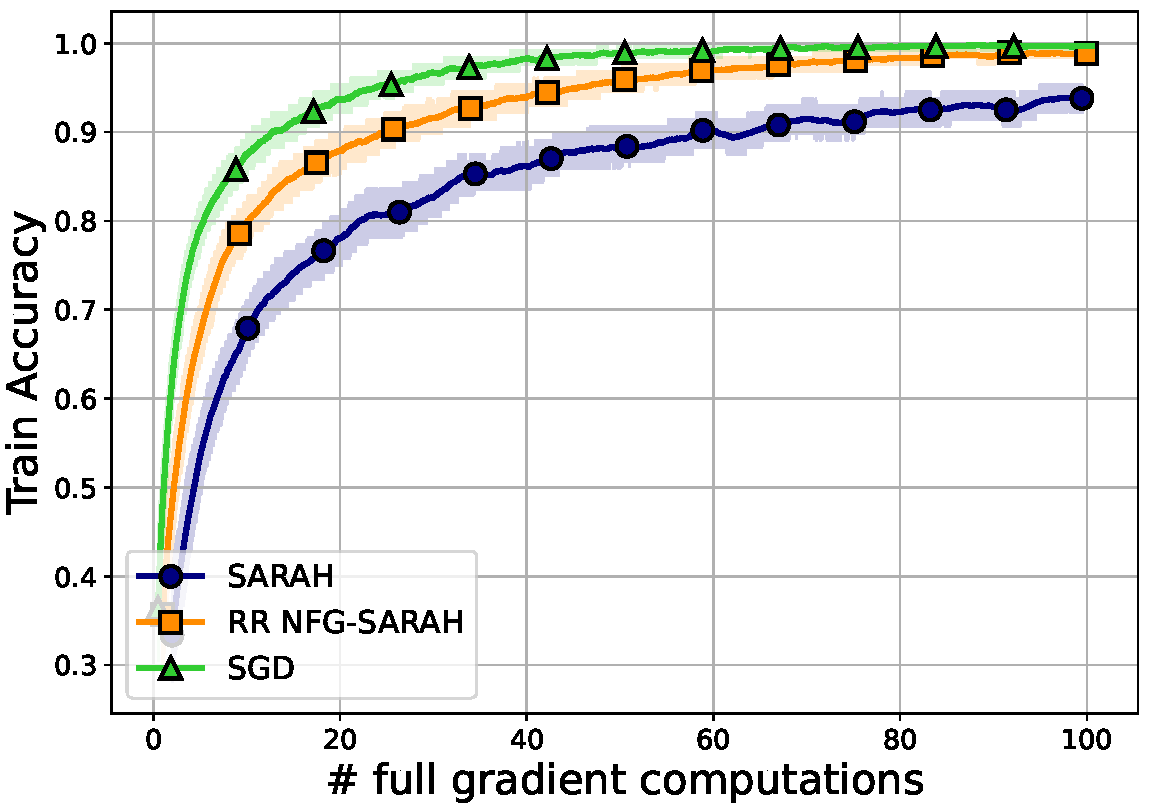
\includegraphics[width=0.45\textwidth]{plots/sarah_10-train-accuracy_compressed.pdf} &
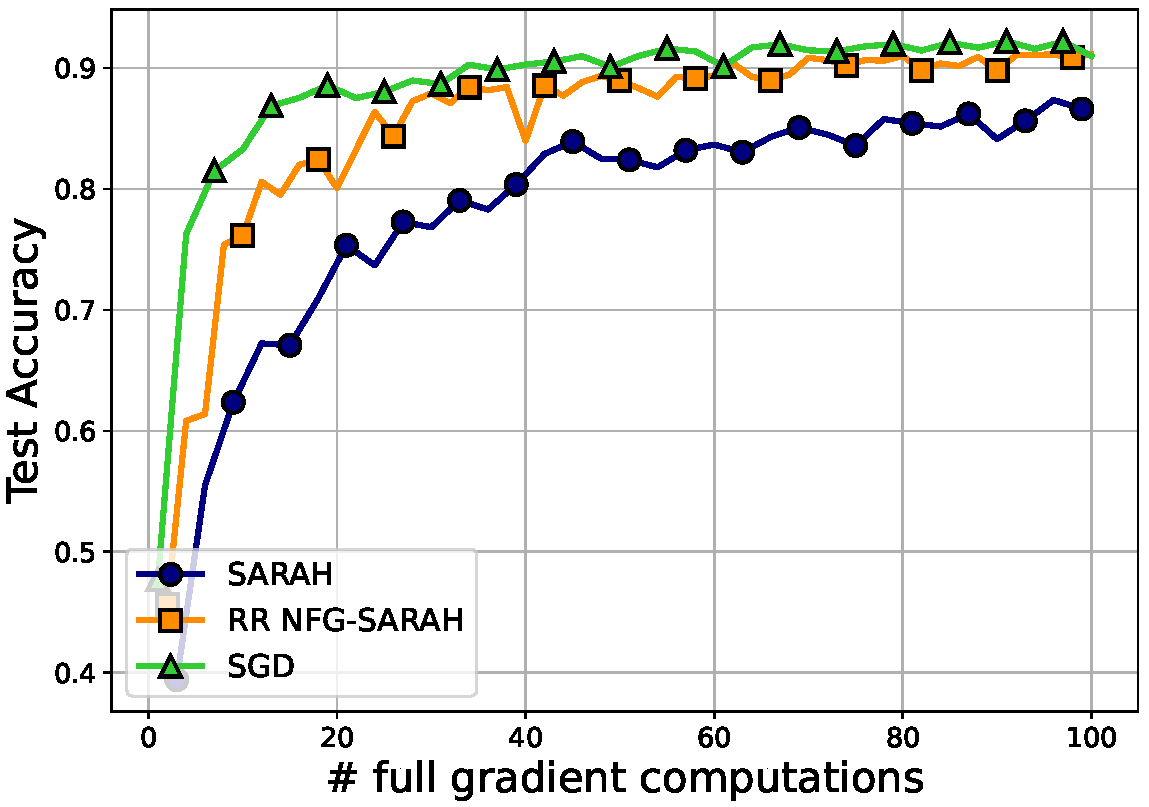
\includegraphics[width=0.45\textwidth]{plots/sarah_10-test-accuracy_compressed.pdf} \\
\end{tabular}
\caption{Сходимость \textsc{No Full Grad SARAH} и классического \textsc{SARAH} на датасете CIFAR-10.}
\label{fig:sarah_10}
\end{figure}

Полученные результаты демонстрируют стабильное убывание функции потерь при обучении методом \textsc{No Full Grad SARAH}, опережая оригинальный алгоритм по скорости сходимости при одинаковом количестве эквивалентных вызовов полного градиента. На тестовой выборке также наблюдается уменьшение функции потерь до более низкого значения, при этом финальная точность постепенно улучшается и достигает более высоких значений на поздних стадиях обучения.

\subsection{Результаты на \textsc{CIFAR-100} с использованием ResNet-18}
\begin{figure}[H]
\centering
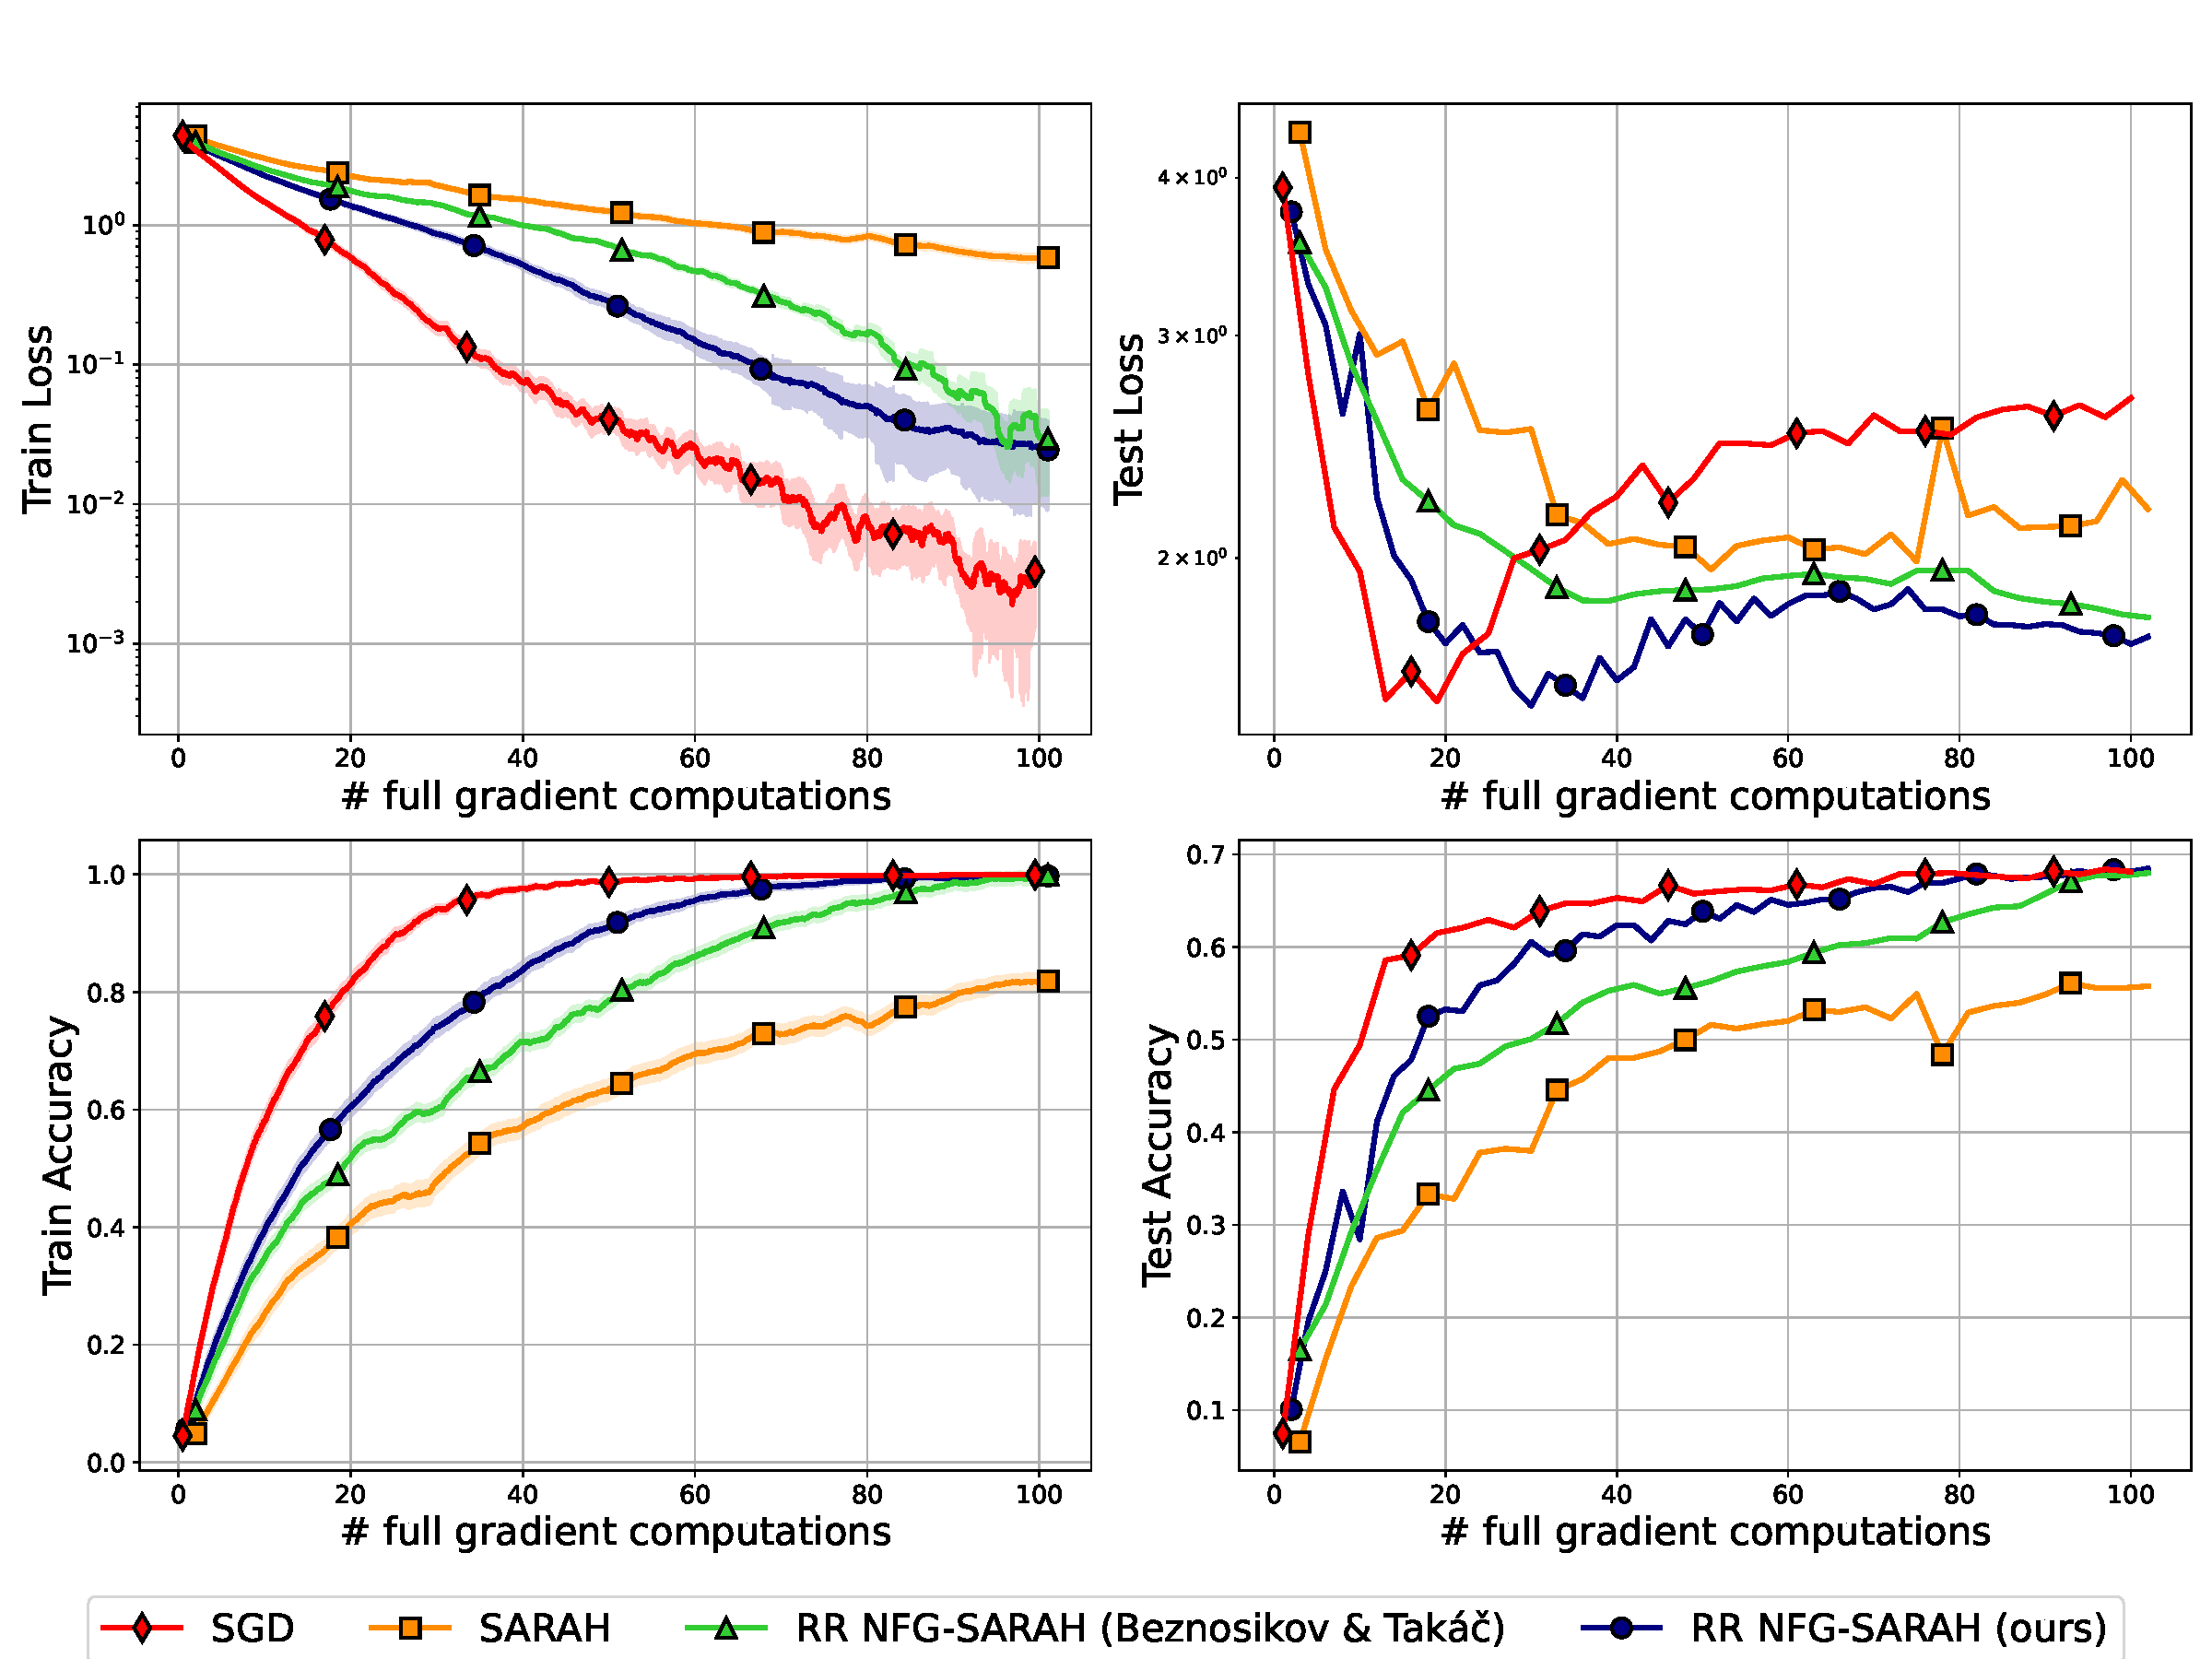
\includegraphics[width=0.8\textwidth]{plots/CIFAR100_LR=0.7_plots_compressed.pdf}
\caption{Сходимость \textsc{No Full Grad SARAH} и \textsc{SARAH} на датасете CIFAR-100.}
\label{fig:sarah_100}
\end{figure}

На CIFAR-100 также была получена устойчивая сходимость предложенного метода. Тестовая ошибка продолжает уменьшаться, даже после того как классический метод достигает минимума. Отметим также, что точность возрастает значительно быстрее на поздних стадиях обучения, что указывает на улучшенное обобщающее поведение.

\subsection{Результаты на Tiny ImageNet с использованием Swin Transformer}

Был использован датасет Tiny ImageNet, включающий 200 классов изображений размером $64\times64$, увеличенных до $224\times224$ с целью соответствия входу модели. Архитектура — Tiny Swin Transformer (\texttt{swin\_T\_patch4\_window7\_224}), инициализированная предобученными весами с ImageNet-1K. Обучение велось с градиентным клиппингом на уровне 1.0. Размер батча — 256.

\begin{figure}[H]
\centering
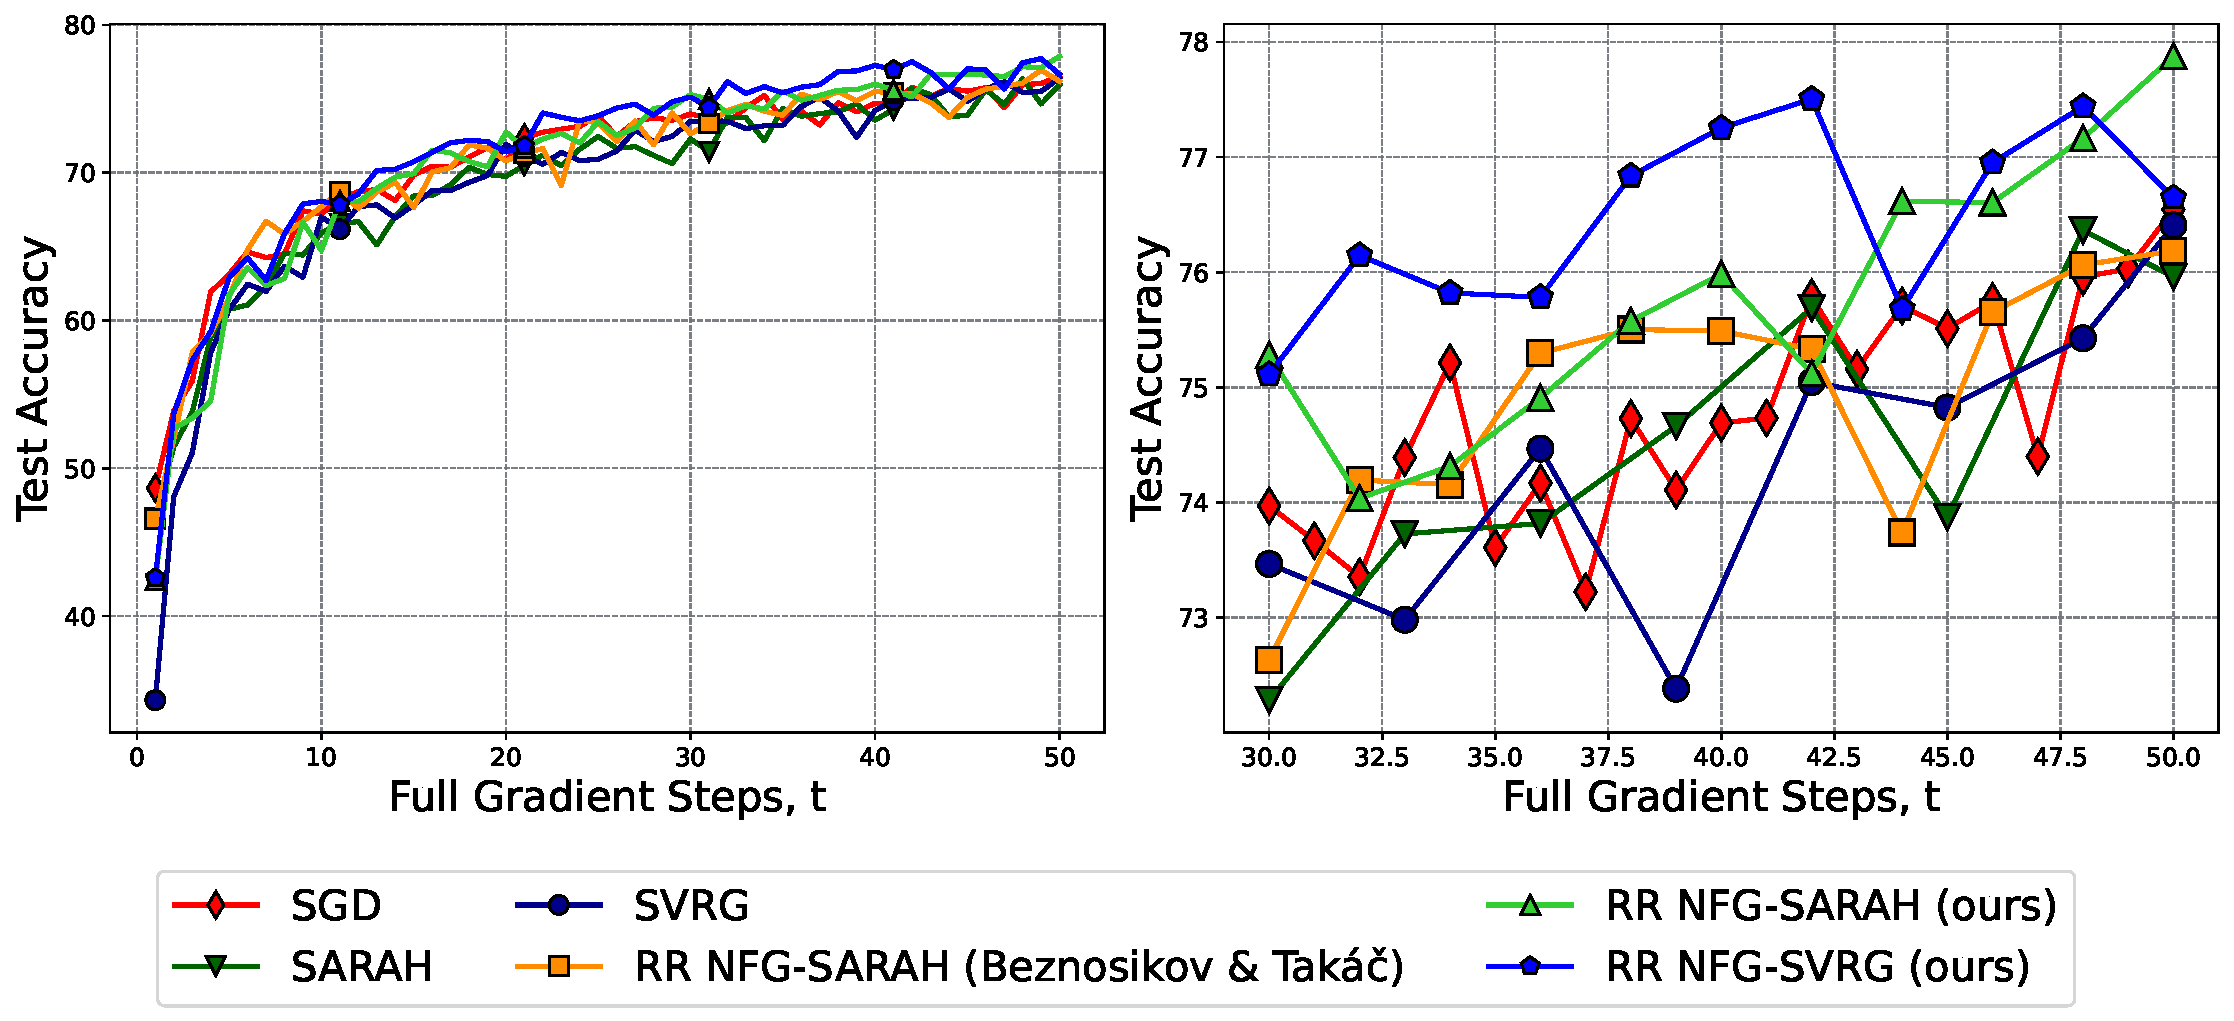
\includegraphics[width=\textwidth]{plots/vit_results.pdf}
\caption{Сходимость \textsc{No Full Grad SARAH} и других методов на Tiny ImageNet.}
\label{fig:swin_plots}
\end{figure}

\begin{table}[H]
\centering
\caption{Финальная точность различных методов на Tiny ImageNet.}
\label{tab:vit}
\begin{tabular}{l|c}
\toprule
Метод & Точность ($\uparrow$) \\
\midrule
\textsc{SGD} & 76.545\% \\
\textsc{SARAH} & 75.961\% \\
\textsc{RR NFG-SARAH} (по \cite{beznosikov2023random}) & 76.186\% \\
\textsc{RR NFG-SARAH} (предложенный) & \textbf{77.875\%} \\
\bottomrule
\end{tabular}
\end{table}

Модифицированный алгоритм \textsc{No Full Grad SARAH}, реализованный в рамках данной работы, демонстрирует превосходство над как классическими, так и ранее предложенными модифицированными алгоритмами. Особенно заметно улучшение в задачах с большим числом параметров и высокой сложностью модели, таких как Swin Transformer.

